\section{為什麼香港的抗爭近年越來越暴力激進?}

嚴格來說,近年來香港的抗爭行動雖然越來越多,但沒有都變得暴力激進。較準確的說法,是一些在數十年來被視為香港抗爭行動共識,如對「和平、理性、非暴力」(簡稱「和理非」)的堅持不再被視為必然,有個別相對大規模而不符合「和理非」原則的抗爭行動出現。此外,社會對相對激進的抗爭行動的理解正在逐漸改變。問題的重點,是過去成就「和理非」原則的社會背景,為何在今天漸漸被認為不合時宜。

從歷史去看,香港的社會抗爭曾有十分激烈的歷史。說回戰前,一九二零年代的海員大罷工和省港大罷工都曾對港英管治帶來威脅。到戰後,一九五六年的雙十暴動與一九六七年的左派暴動,都做成嚴重的社會混亂和平民傷亡。不過在六七暴動後,暴力抗爭成為社會禁忌。從八十年代末到二零一零年代中期,各種抗爭行動的組織者為免被貼上「搞亂香港」的標籤,一般都會很有意識的避免激烈衝突,即使個別示威中與警方有所推撞,也是以點到即止的形式發生,為了爭取傳媒注意多於真的要衝破警方防線。

至於一些大型的群眾活動,則更往往以其自律約束作為道德感召力的依據。例如每年維園六四晚會過後,都會有參與者自發留下幫忙清理垃圾。而二零零三年的七一遊行過後,不少評論均以「五十萬人上街卻沒有打翻一個垃圾筒」和「沿途商舖毫不擔心照常營業」等的觀察來讚賞參與者的克制。到了二零一四年佔領運動,事件最受到國際輿論的讚揚的角度正是參與者均有禮待人,佔領區有市民自發設置資源回收點,有大學講師和中學老師在佔領區架起書桌為學生免費補習,外國記者紛紛表示從來沒有報道過如此和平及讓他們感到安全的大型反抗運動。

\begin{figure}[htbp]
    \centering
    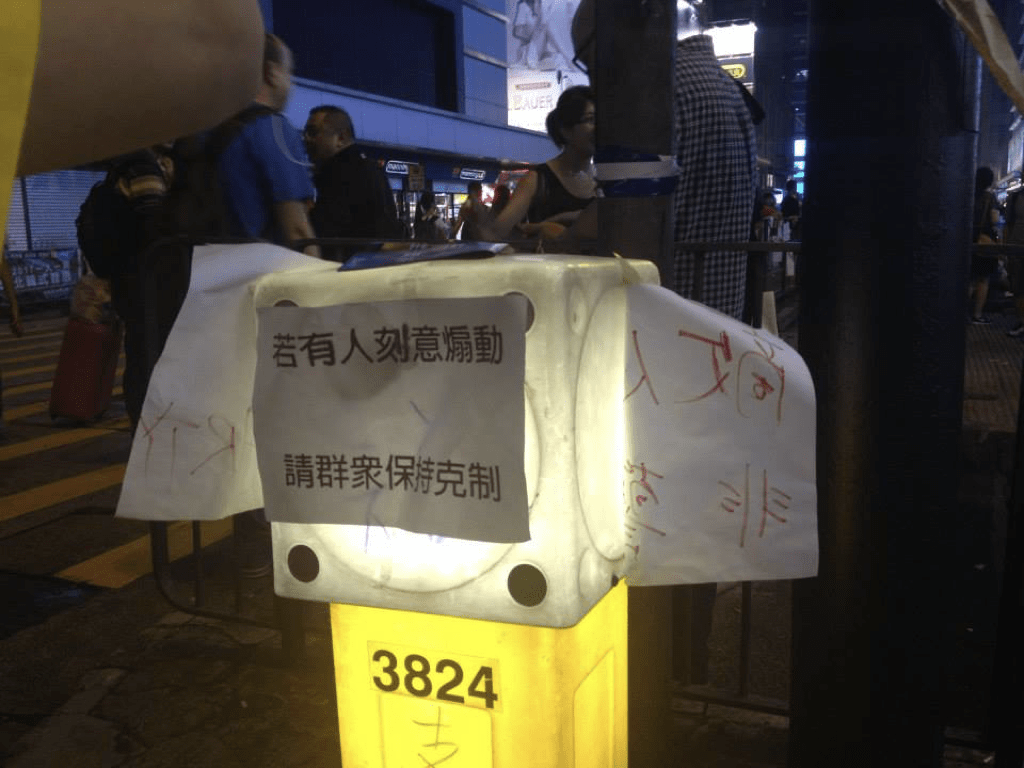
\includegraphics[width=0.7\textwidth]{c31/h-klesson1-049.png}
    \caption{佔領運動初期,有市民自發在佔領區呼籲冷靜和不要視警察為敵人} 
\end{figure}

組織者對「和理非」(有時還要加上「非粗口」,即「和理非非」)的堅持,很大程度上出於他們相信如能號召越多的市民參與其中,成功的機會就越大;而要讓更多的人參與,就要使用大多數人都接受的方式。回顧過去案例,二零零三年七一遊行的參與人數遠超預期,成功拉倒了《基本法》第二十三條的立法。縱觀國際,組織者也會援引美國六十年代黑人平權運動等的案例,以支持對非暴力抗爭的堅持。此外,八九民運以武力鎮壓結束,也讓不少組織者深信要透過堅持非暴力來避免流血衝突,不給予政府籍口強制介入。

也有一些組織者不甘於主動避免任何衝突,例如二零零六至二零零七年期間的保留舊中環天星碼頭和皇后碼頭事件,就是以行動者以直接行動的方式阻擋清拆工程。在天星碼頭事件中,行動者直接闖入地盤阻止工程車輛運行;在皇后碼頭事件,行動者則在該處露宿露宿留守超過半年,阻延政府動工清拆。不過嚴格來說,他們採取的直接行動只限於對場地的佔領,沒有攻擊任何人,不算暴力抗爭。但他們的行為在當時社會環境當中仍受到不少質疑,對他們的抗爭方式的議論甚至蓋過了目的本身。

社會形勢改變迅速,比天星皇后更激烈的抗爭行動相繼出現,當年被認為走得太前的組織者在新形勢下反而被批評為不夠激進。近年明顯被認為是激進甚至是暴力的抗爭行動,有二零一二年起多次的光復行動,以及二零一六年農曆年期間的旺角騷亂。

二零一二年起多次的光復行動,都發生在中國大陸遊客和水貨客與本地居民日常生活衝突較多的地方,包括沙田、上水、屯門和元朗。組織者認為中國大陸遊客和水貨客過多,使得本地居民的日常生活受嚴重威脅,因此要把這些地方從外來影響中「光復」過來。具體的抗爭行為,包括阻礙專門服務中國大陸遊客和水貨客的商店,貼身追蹤他們懷疑是中國大陸遊客或水貨客的個人,向對方辱罵甚至破壞他們的隨身物品,如踢翻行李箱。這些針對個人的攻擊行為過去甚少在香港的抗爭中出現,在主流傳媒受到廣泛討論及批評。

說到激烈衝突引發的社會震盪,最具代表性者莫過於二零一六年農曆年期間的旺角騷亂。農曆年期間無牌熟食小販在街頭擺檔,是一個香港庶民文化傳統。不過近年政府執法趨嚴,在本土思潮下往往被理解為文化打壓。二零一六年農曆年初一晚上,政府管理人員和支持小販的組織之間發生衝突,演變成近年罕見的騷亂場面。期間有人向警察投擲雜物,有警察向天開槍示警;又有人搬起路障和推放雜物縱火,混亂持續至第二天早上。事件引發公眾嘩然,既有批評參與者使用暴力,也有譴責警方的處理手法。事後警方大規模搜捕涉案人士,多位參與者被判暴動罪成。

光復行動和旺角騷亂,在香港的眾多抗爭行動來說算是異數,絕大多數仍然堅持以「和理非」的方式進行。不過從論述層面來說,社會中對抗爭行動的理解近年來確實有所改變,「和理非」不再是絕大多數組織者都堅持的底線,甚至成為新一批組織者所嘲諷。「勇武」一說的流行,使相對激烈的抗爭方式愈來愈被特別是年輕人所接受。

對於這些改變,非建制陣營中傳統的政治代表初時選擇了劃清界線,也就是所謂的「割席」,引發非建制陣營的進一步分裂。在比例代表制的選舉制度下,由於市民對抗爭活動應否走向激進也意見不一,政治人物的不同取態實為立法會本身碎片化的一個表徵(見問題二十二)。不過,也有個別的政治人物和評論者在不認同激烈抗爭方式的同時,對有人會選擇這些方式表示諒解,並願意為他們面對司法後果時提供支援。可想像,這種立場不易把握,甚至不時會變成裡外不是人。

總的來說,激進抗爭的出現和前文提及的議會激進化有不少相似之處。在議會中,由於在野政團持久處於在野位置,越來越難說服支持者審慎妥協可帶來改變,政團之間的團結誘因也續步降低。在議會以外,同樣的過程也在抗爭組織之間發生,參與者有意或無意間不再相信合作可以變得壯大,約束各組織者的不成文共識越來越容易被打破,新出現的組織者也不覺得有需要和過去的組織者協調,甚至認為他們過去的共識正正是他們未能成功的原因,於是鼓催要「拆大台」,要求抗爭運動全面的去中心化。換言之,要理解激進抗爭的出現,不能只把焦點僅僅放在行動者本身,也要看他們如何理解所處的時代背景。

說到「和理非」受到挑戰的時代背景,學者沈旭暉早於二零一一年便在一篇文章中論及。當時他回應時任政務司長的唐英年對年青人走向激進的批評,認為應理解過去香港強調「和平理性」並非「與生俱來」而有其獨特的時代背景。他提到六七暴動後,麥理浩推行福利社會,為香港人信任漸進改革帶來基礎;社會發展迅速加上政府尊重專業,也讓香港人相信制度和願意在制度內尋求改變。反過來說,當社會寧願在制度外作激烈抗爭,其實代表原有制度內的通道已被阻塞。

沈文出版之時,對「和理非」的批評其實尚未成形,部份抗爭者對「和理非」的失望要到往後其他事件的發生後才變得普遍。其中二零一四年的佔領運動,對此很可能起了關鍵作用。佔領運動原自「讓愛與和平佔領中環」的倡議,起始組織者十分強調以和平方式感召更多人參與,和避免其他人混入破壞。到了佔領運動全面爆發,參與者平來尚以「和理非」抗爭為榮,唯及後與警方的衝突變得激烈,警方濫權的情況引發公憤(如「七警案」,見問題三十),而歷時七十九日的佔領運動未能迫使中央政府撤回為普選設限的「八三一決定」,也使得「和理非」抗爭對一些抗爭者的感召力大為減退。

由此開始,社會對何謂暴力抗爭的理解也逐漸改變。帶同攻擊性武器主動攻擊別人,當然算是暴力;但帶同防護裝備讓自己在被警方驅趕時可作抵禦,又應如何理解?如果一個活動本來沒有預謀或意圖引致混亂,但在警方或保安反應的過程中引發混亂甚至有人受傷,那麼行動者本身是否需要負責?如果行動者只針對濫權的警隊,而且行動前主動呼籲其他市民離開,又能否接受?當警察暴行越來越猖狂,不少行動者都認為作出一定防護是必然的選擇。此外,激烈抗爭本身的沉重代價,無論是肉體上損傷或是數以年計的牢獄生涯,亦成為另一種的抗爭精神感召。過去數年來,每次衝突當中各種微細但重要的差別,引發不少對於何謂暴力的社會討論,一方面讓支持激進手段的行動者有機會反思其方式,另一方面社會整體對激進抗爭的接受程度亦慢慢改變。

這些改變會帶來甚麼後果?第一種可能,是「和理非」和「勇武」的支持者互不信任,認為對方拖了自己的後腿。號召衝擊的,會被溫和一方指責是受北京指使的潛伏者,要刻意搞散運動;在集會唱歌打氣的,會被激進一方指責是搞「卡拉OK社運」,把抗爭現場變成嘉年華會。由這些互相攻擊所引發的矛盾是佔領運動後香港公民社會陷入低潮的一個主要原因。

第二個可能,是雙方理慢慢解到各自在運動中有其角色,在「雙向互不割席」的前提下實行「各有各做」,甚至實現某種程度的互相補足。這種默契在《逃犯條例》修訂的抗爭中十分明顯,無論選擇在警察面前拿雨傘擋胡椒液體,還是連續整晚唱詩歌緩和氣氛,都被接納為運動的一部分。有評論指佔領運動後經過數年的沉殿,公民社會對成效問題有較成熟的取態。而由於警察暴行的惡劣程度遠遠不乎比例,使「和理非」和「勇武」有條件站在同一陣線予以譴責。

\begin{figure}[htbp]
    \centering
    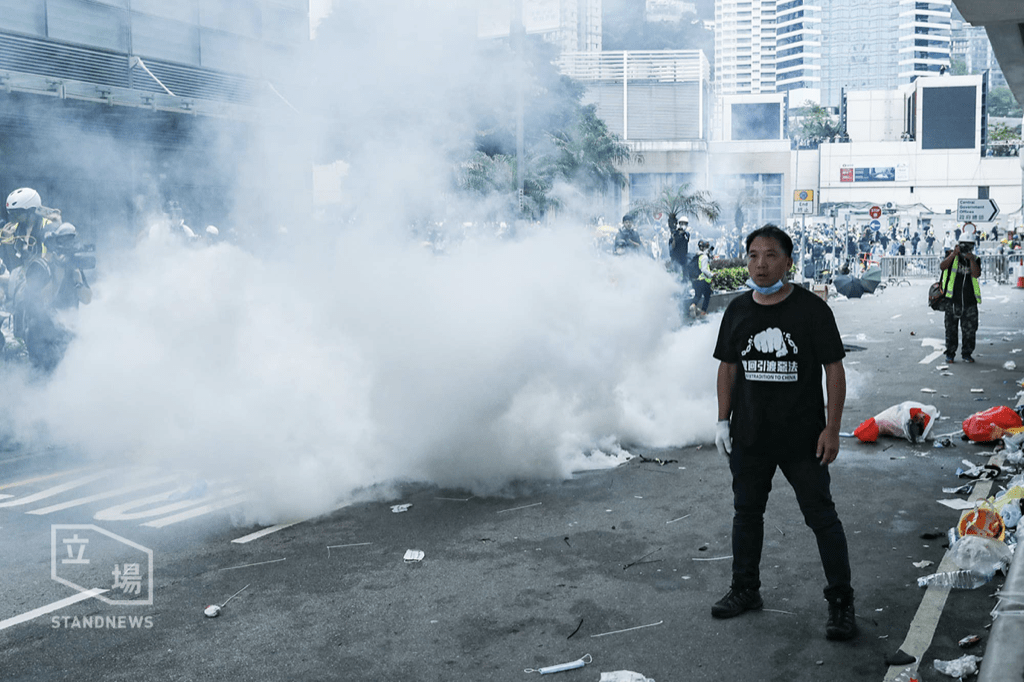
\includegraphics[width=0.7\textwidth]{c31/h-klesson1-050.png}
    \caption{一般被認為立場溫和的民主黨主席胡志偉於「反送中」抗爭街頭} 
\end{figure}

總的來說,激進甚至暴力抗爭的出現是社會失衡的徵兆,而正如譴責一個病人發燒是不能協助他更快痊癒,要問的是香港為何出現了一系列的管治失效。前文提到行政長官的管治認授本身就有先天缺陷,然而本來用來補救的措施如管治聯盟和政治任命官員等又未能有效運用,反過來進一步拖低政府的管治威信。過去政府會通過吸納專家學者來增加管治認授,但在效忠先行的年代卻越來越多專業人士被推向制度以外。行政權失效,正常來說公眾可通過立法權來監督,但同樣正如前文所述,立法權也明顯地被逐步肢解,無論實權或威信都在一步一步流失。來到司法權,無論是執法機關和檢控部門的中立性和專業性都越來越受質疑,法庭本身的訟裁地位又因釋法的猜測而被削弱。從制度內走到制度外,主流傳媒和傳統公民社會團體的能力又不斷被壓制。上述的眾多機制,本來的都是吸納社會壓力和將之轉化為改革動力的方式。當這些機制逐一失效,不代表背後的社會厭力就會消失。相反,因為社會厭力無法轉化成對社會有益的改革動力,則往往只好以更激烈的方式出現。直接點說,激烈抗爭的出現,很大程度上是時勢迫出來的。

最後,應注意走向激進暴力的並不限於抗爭行動,建制陣營也學會了發動所謂的群眾運動去支持自己,甚至不介意動用激烈的言語甚至行為來攻擊其他人。例如二零一七年初時任立法會議員的羅冠聰就在香港機場被多名自稱親中人士推撞襲擊,使其身上多處受傷。各式比傳統建制陣營更為激進的「愛國團體」相繼湧現,目的不一定是要說服別人加入他們的陣營,只要能讓公眾對所有的政治參與生厭,已足以達到維持現狀的目的。說到這兒,不難懷疑建制陣營雖然聲稱反對激烈的抗爭方式,實際上卻可能樂於社會出現這種走向。畢竟,當抗爭方式走向激烈,打壓的方式也可以來得更粗糙,增加普羅大眾參與其中的成本。

伸延閱讀:

\href{https://theinitium.com/article/20150921-hongkong-occupycentraloneyear02/}{林怡廷(2015):〈旺角少年,不被理解的戰鬥〉,《端傳媒》2015年9月26日}

沈旭暉(2011): 〈八月飛霜 如何再造和平理性的土壤﹖〉,《明報》2011年9月5日。

Garrett D and Ho WC (2014) Hong Kong at the Brink: Emerging Forms of Political Participation in the New Social Movement, in Cheng JYS (ed) \textit{New Trends of Political Participation in Hong Kong}. p347-384

網上資源:
\href{http://thestand.news/politics/6-12-佔領-圖輯二-金鐘攻防戰-雨傘口罩抗橡膠彈催淚彈/}{立場報道(2019)金鐘攻防戰 雨傘口罩抗橡膠彈催淚彈,2019年6月12日}